\section{Python basics}
\label{sec:python_basics}

\begin{frame}
	\frametitle{A recap of python skills}
	\framesubtitle{Image from ThinkPython}
	\begin{center}
		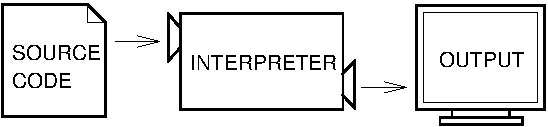
\includegraphics[width=0.8\textwidth]{figures/interpret.pdf}
		%https://github.com/AllenDowney/ThinkPython/blob/master/book/figs/interpret.pdf
	\end{center}
\end{frame}

\begin{frame}
	\frametitle{Starting at the basics}
	\lstinputlisting{code/summing_range.py}	
	\pause
	\begin{columns}
		\column{0.455\textwidth}
		\begin{questionblock}{Let's get warmed up}
			What does this compute?	
			\begin{multicols}{2}
				\begin{enumerate}[A.]
					\item $\sum\limits_{i=0}^{m} i$
					\item $\sum\limits_{i=m}^{u} i$
					\item $\sum\limits_{i=m}^{u+1} i$
					\item I don't know
				\end{enumerate}
			\end{multicols}
			\vspace*{0.2cm}
		\end{questionblock}
		\column{0.455\textwidth}
		\pause
		\begin{answerblock}{}
			It sums all numbers from $m$ up to $u$: Answer B.
		\end{answerblock}
	\end{columns}
\end{frame}

\begin{frame}
	\frametitle{Let's make that more computer sciencey}
	\only<3->{\framesubtitle{Why use a for-loop?}}
	We should add typing information:
	\lstinputlisting{code/summing_range_typing.py}	
	\pause
	\begin{questionblock}{Why?}
		Why should we add typing information?
	\end{questionblock}

	\pause
	We can do without the for-loop:
	\lstinputlisting{code/summing_range_nofor.py}	
\end{frame}

\begin{frame}
	\frametitle{Creating a new list}
	\begin{overlayarea}{\textwidth}{\textheight}
		\only<3->{
			We can do even more by using \textit{list comprehensions}
		}
		\only<1,2>{
			\lstinputlisting{code/cumsum.py}	
		}
		\only<3>{
			\lstinputlisting{code/cumsum_typed.py}	
		}
		\only<4->{
			\lstinputlisting{code/cumsum_comprehension.py}	
		}
		\only<2>{
			\begin{questionblock}{More typing}
				What typing information should we add here?
					\begin{enumerate}[A.]
						\item \texttt{def fey(my\_list: int) -> int:}
						\item \texttt{def fey(my\_list: List[int]) -> int:}
						\item \texttt{def fey(my\_list: List[int]) -> List[int]:}
						\item I don't know
					\end{enumerate}
				\vspace*{0.2cm}
			\end{questionblock}
		}
		\only<5>{
	\begin{block}{List comprehensions}
		A list comprehension allows for a one-liner to create a full list based on another list.\\
		We will use it in our code snippets and samples (also in the homework).\\
		You can use a regular for-loop in your solutions if you prefer!
	\end{block}	
		}
	\end{overlayarea}
\end{frame}

\begin{frame}
	\frametitle{On the subject of classes}
	\framesubtitle{Object-oriented Python}

	\pause
	\begin{columns}
		\column{0.705\textwidth}
	\lstinputlisting[]{code/simple_classes.py}
	\pause
			
		\column{0.305\textwidth}
			
	\begin{questionblock}{What does the code print?}
			
	\begin{enumerate}[A.]
		\item Butz\\
			Fey Powers
		\item 1\\
			3
		\item Nothing, the code will give (an) error(s).
		\item I don't know.
	\end{enumerate}
	\end{questionblock}
	\end{columns}
\end{frame}
